\iffalse
\KIHON	{基本を確認しておこう}
\KIHON2 {基本問題を解いてみよう}
\REI {例}
\KAI {解}
\REIDAI {例題}
\KAITOU {解答}
\KAISERU {解説}
\MONDAI {問題}
\fi

\chapter{○○○○○○○}
\newcommand\Binom[2]{\bigg(\begin{array}{@{\,}c@{\,}}#1\\[-.5mm]#2\end{array}\bigg)}

\section{○○○○}
\step{基本を確認しておこう}


○○○○○○○○○○○○○○○○○○○○○○○○

\begin{enumerate}
\item[a.] ○○○○
\item[b.] ○○○○
\item[c.] ○○○○
\end{enumerate}
\begin{titlebox}{○○○○}
$\begin{array}{ll}
\text{○○○○○○○○}&\Longleftrightarrow P(a)=0\\
\text{○○$P(x)$○○$ax-b$○○}&\Longleftrightarrow P\left (\frac{b}{a}\right )=0
\end{array}$\\
\end{titlebox}
\begin{例}
$P(x)=2x^{3}-7x^{2}+6x+5=0$ ○○○○○○○○.
\end{例}
\begin{解}
○○$x=\frac{b}{a}$($a$ ○ $b$ ○○○○○○○○,$a$ ○○○○○○,$b$ ○○)○○○○○○○,$x=\pm\frac{P(x)\text{○○○○○○○○○}}{P(x)\text{○○○○○○○○○○○○}}$ ○○○○○○○○○.

\noindent
$x=\pm\frac{\text{5○○○○○}}{\text{2○○○○○}} =\pm\frac{1,5}{1,2}$ ○○ $x=\pm 1, \pm 5, \pm\frac{1}{2}, \pm\frac{5}{2}$ ○○○○
\[
P\left (-\frac{1}{2}\right )=2\cdot\left (-\frac{1}{8}\right )-7\cdot\frac{1}{4}+6\cdot\left (-\frac{1}{2}\right )+5=-2-3+5=0
\]%%\newpage
\begin{Mw}{40mm}{%
%\arraycolsep.5zw$
%\begin{array}{rrrrr}
%\multicolumn{1}{r|}{-\dfrac{1}{2\rule[-1mm]{0pt}{0pt}}}&2&-7&6&5\\
%\cline{1-1}
%&&-1&4&-5\\
%\hline
%&2&-8&10&\multicolumn{1}{|r}{0}\\
%\cline{5-5}
%\end{array}$
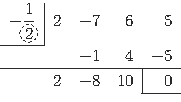
\includegraphics{./fig/fig00-step01}
}
○○○○○
\begin{align*}
P(x)&=\left (x+\frac{1}{2}\right )(2x^{2}-8x+10)\\
&=(2x+1)(x^{2}-4x+5)=0
\end{align*}
○○○,$x=-\frac{1}{2},\ 2\pm i$
\end{Mw}

{\footnotesize
○○○○○○,$x$○○○○1○○$x-\alpha$○○○○○○○○○○○○○○○○○○,「○○○○」○○○○○.
○○○○,「$(x^3-3x+2)\div(x-2)$○○○○○○?」○○○,
○○○$x-2$○0○○○$x={\fboxsep.1zw\colorbox[gray]{.9}{$2$}}$○○○○○○\,{\fboxsep.1zw\colorbox[gray]{.9}{$1 \quad 0 \quad -3 \quad 2$}}\,○
\[
\raisebox{0pt}[0pt][0pt]{\def\arraystretch{0.85}\begin{array}[t]{@{\ }c@{\ }|}%
\rule{0pt}{1.5ex}2\\[0pt]\hline
\end{array}} \quad 1 \quad 0 \quad -3 \quad 2
\]
\begin{Mw}(0pt,9mm){48mm}{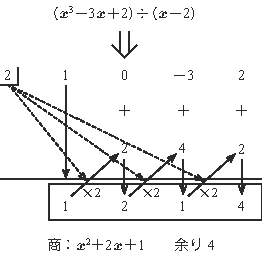
\includegraphics{./fig/sec00_betsu01.pdf}}
\noindent
○○○○○○○○○○○○○○.
○○○○○

\vspace{.5\baselineskip}
1. 1○○○○$\Rightarrow$\ajKaku{1}

2. $\ajKaku{1}\times 2\Rightarrow2$

3. $0+2\Rightarrow$\ajKaku{2}

4. $\ajKaku{2}\times 2\Rightarrow4$

5. $(-3)+4\Rightarrow$\ajKaku{1}

6. $\ajKaku{1}\times 2\Rightarrow$2

7. $2+2\Rightarrow$\ajKaku{4}(○○)

\vspace{.5\baselineskip}
\noindent
○○○○○○○○○,○○○○○○○○○○○○○○○○○.
○○○○○$P(x)=0$○○○○,$P(\alpha)=0$○○○$\alpha$○○○○○,○○○○○○○○○,$P(x)=(x-\alpha)P_1(x)=0$○○○○○○○○○○,○○○○○○○○.
\par
\end{Mw}
}

\end{解}
\step{基本問題を解いてみよう}
\begin{例題}
○○○○○○○○○○.
\begin{longtable}[l]{@{}l@{\hskip4zw}l}
(1)\hspace{1zw}$2x^{3}-x^{2}-13x-6=0$\hspace{4zw}&
(2)\hspace{1zw}$3x^{3}-4x^{2}+2x+4=0$ \\
 (3)\hspace{1zw}$x^{4}-4x+3=0$&
\end{longtable}
\end{例題}

\begin{解答}
○○○○○○○ $P(x)$ ○○○.\\[3mm]
\begin{fleqn}[4zw]
(1) $\Mframe{P(-2)}=-16-4+26-6\,\Mframe{=0}$\Footnote{○○○○○○○○$x=\pm\frac{-6\text{○○○○○}}{\text{2○○○○○}}=\pm\frac{1,2,3,6}{1,2}$}\\
$P(x)$○$x+2$○○○○,○○ $2x^{2}-5x-3$
\[
P(x)=(x+2)(2x^{2}-5x-3)=(x+2)(2x+1)(x-3)=0
\]
○○○,$x=-2, -\frac{1}{2},3$\kotae
\end{fleqn}

\begin{fleqn}[4zw]
(2) $P\left (-\frac{2}{3}\right )=3\cdot\left (-\frac{8}{27}\right )-4\cdot\frac{4}{9}+2\cdot\left (-\frac{2}{3}\right )+4=0$\\
\hspace{1zw}$P(x)$○$3x+2$○○○○,○○ $x^{2}-2x+2$
\begin{alignat}{1}
P(x)=(3x+2)(x^{2}-2x+2)=0\notag
\end{alignat}
○○○,$x=-\frac{2}{3}, 1\pm i$\kotae
\end{fleqn}
\begin{fleqn}[4zw]
(3) $P(1)=1-4+3=0$\\
$P(x)$○$x-1$○○○○,○○ $Q(x)=x^{3}+x^{2}+x-3$
\begin{alignat}{1}
P(x)=(x-1)(x^{3}+x^{2}+x-3)\notag
\end{alignat}
○○○ $Q(1)=1+1+1-3=0$ ○○○
\begin{alignat}{1}
Q(x)=(x-1)(x^{2}+2x+3)\notag
\end{alignat}
○○○○○
\begin{alignat}{1}
P(x)=(x-1)^{2}(x^{2}+2x+3)\notag
\end{alignat}
○○○,$x=1$ (2○○),\ $-1\pm\sqrt{2}i$\kotae
\end{fleqn}
\end{解答}

\vspace{.5\baselineskip}\noindent
\begin{center}
{\footnotesize
\begin{tabular}{@{}c@{}}\tabcolsep.75\tabcolsep
(1)\ \begin{tabular}[t]{>{$}r<{$}>{$}r<{$}>{$}r<{$}>{$}r<{$}>{$}r<{$}}
\multicolumn{1}{r|}{$-2$} & 2 & -1 & -13 & -6\\
\cline{1-1}
   &   & -4 &  10&  6\\
   \hline
   & 2 & -5 &\multicolumn{1}{r|}{$-\phantom{1}3$}&  0\\
   \cline{5-5}
\multicolumn{5}{l}{○ $2x^2-5x-3$}
\end{tabular}\quad\hskip2mm
(2)\ \begin{tabular}[t]{>{$}r<{$}>{$}r<{$}>{$}r<{$}>{$}r<{$}>{$}r<{$}}
\multicolumn{1}{r|}{$-\dfrac{2}{3}$} & 3 & -4 & 2 & 4\\[2mm]
\cline{1-1}
\multicolumn{5}{r}{}\\[-6.5mm]
   &   & -2 & 4&  -4\\
   \hline
   & 3 & -6 &\multicolumn{1}{r|}{$6$}&  0\\
   \cline{5-5}
\multicolumn{5}{l}{○ $x^2-2x+2$}
\end{tabular}\quad\hskip2mm
(3)\ \begin{tabular}[t]{>{$}r<{$}>{$}r<{$}>{$}r<{$}>{$}r<{$}>{$}r<{$}>{$}r<{$}}
\multicolumn{1}{r|}{$1$} & 1 & 0 & 0 & -4 & $3$\\
\cline{1-1}
   &   & 1 & 1 &  1 & -3 \\
\hline
\multicolumn{1}{r|}{$1$} & 1 & 1 & 1 & \multicolumn{1}{r|}{$-3$} & 0\\
   \cline{1-1}\cline{6-6}
& & 1 & 2 & 3 & \\
\cline{1-5}
&  1 & 2 &\multicolumn{1}{r|}{$3$} &0 &\\
\cline{5-5}
\multicolumn{6}{@{}l}{\hbox to2zw{\rule{0pt}{1.2zh}○ $x^2+2x+3$}}
\end{tabular}
\end{tabular}
}
\end{center}

\vspace{-4mm}
%%\clearpage
\section{○○○}
\step{基本を確認しておこう}

%\begin{Mw}<6>[+3]{35mm}{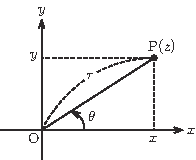
\includegraphics{./fig/sec00_2_1.pdf}}
○○○○○○,$0$ ○○○○○○ $z=x+yi$
○○○○○ $\mathrm{P}$ ○○,$\overrightarrow{\OP}$ ○○○○○○○○○○○○○
○ $\theta$, $\overline{\OP}$ $=|z|=r$ ○○○○
\[
 x=r\cos\theta,\ y=r\sin\theta
\]

\begin{fleqn}
\[
\text{○○○○,}\ z=r(\cos\theta+i\sin\theta)\hspace{1zw}(r>0)\tag*{……①}
\]
\end{fleqn}\pagebreak[3]


\begin{Mw}[+1]{35mm}{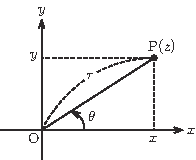
\includegraphics{./fig/sec00_2_1.pdf}}
\hspace*{-1zw}○○○○○.①○○○○○○○○,○○○ $z$ ○\textbf{○○○}○○○.$r$ ○ $z$ ○○○○,$\theta$ ○ $z$ ○\textbf{○○}○○○,$\arg z$ ○○○.$\arg$○argument ○○○○○.
\[
r=|z|,\hspace{1zw}\theta=\arg z
\]
\textbf{[1]}\hspace{1zw}\textbf{○○}\hspace{1zw}○○○ $z$ ○○○○,$\overrightarrow{\mathrm{OP}}$ ○○○○○○○○○○○○○○○○○○○○○,○○○○○○○○○○○○.$\theta$ ○ $z$ ○1○○○○○○
\[
\theta+2 n\pi \hspace{1zw} (n=0, \pm 1, \pm 2, \ldots)
\]
○○○○$z$○○○○○○,○○,$z$○○○○○○○○○○○○○.
\end{Mw}

○○,$z=0$ ○○○○○○○○○○○○○,$\arg 0$ ○○○○○○○○○○.
○○○,$z=r(\cos\theta+i\sin\theta)$ ○○○
\[
\overline{z}=r(\cos\theta-i\sin\theta)=r\{\cos(-\theta)+i\sin(-\theta)\}
\]
○○○\hspace{3zw} $|\overline{z}|=|z|$\hspace{1zw}○○\hspace{1zw}$\arg\overline{z}=-\arg z$

\begin{fleqn}
\begin{alignat*}{1}
\text{2○○○○○} z_{1}=r_{1}(\cos\theta_{1}+i\sin\theta_{1}) , z_{2}=r_{2}(\cos\theta_{2}+i\sin\theta_{2})\tag*{……②}
\end{alignat*}
\end{fleqn}


\noindent
○○○\hspace{2zw}$z_{1}=z_{2}\hspace{1zw}\Longleftrightarrow\hspace{1zw} r_{2}=r_{1}$ ○○ $\theta_{2}=\theta_{1}+2n\pi\hspace{1zw}(n\in \mathbb{Z})$

\noindent
\textbf{[2]}\hspace{1zw}\textbf{○○○○○○・○○}\hspace{1zw}②○○○○2○○○○○ $z_{1}$, $z_{2}$○○○○
\begin{fleqn}[4zw]
\begin{alignat}{1}
z_{1}z_{2}&=r_{1}(\cos\theta_{1}+i\sin\theta_{1})\cdot r_{2}(\cos\theta_{2}+i\sin\theta_{2})\notag\\
&=r_{1}r_{2}\{(\cos\theta_{1}\cos\theta_{2}-\sin\theta_{1}\sin\theta_{2})\notag\\
&\phantom{=\;} +i(\sin\theta_{1}\cos\theta_{2}+\cos\theta_{1}\sin\theta_{2})\}\notag
\end{alignat}
\end{fleqn}
\hspace{0zw}$\text{○○}\hspace{2zw}\quad z_{1}z_{2}=r_{1}r_{2}\{\cos(\theta_{1}+\theta_{2})+i\sin(\theta_{1}+\theta_{2})\}$

\noindent
\begin{fleqn}
\begin{alignat*}{3}
\text{○○○○}&\hspace{3zw}&&|z_{1}z_{2}|= |z_{1}||z_{2}|,\ \arg(z_{1}z_{2})=\arg z_{1}+\arg z_{2}\tag*{……③}
\end{alignat*}
\end{fleqn}
○○○○○\hspace{2zw}$\left |\frac{z_{1}}{z_{2}}\right |=\frac{|z_{1}|}{|z_{2}|},\hspace{1zw}\arg\left (\frac{z_{1}}{z_{2}}\right )=\arg z_{1}-\arg z_{2}$\hspace{2zw}○○○○○.

\pagebreak
\step{基本問題を解いてみよう}
\begin{例題}
○○○○○○○○○○○○.\par
\begin{longtable}[l]{@{}l@{\hskip4zw}l}
(1)\quad$z=-\frac{5}{2}i\ $&$(2)\quad z=\frac{-5+i}{2-3i}$
\end{longtable}
\end{例題}

\begin{解答}
%\begin{Mw}{26mm}{\Fig{26mm}{24mm}}
\begin{Mw}{26mm}{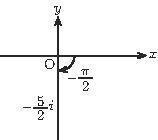
\includegraphics{./fig/sec00_2_2.pdf}}
(1)\hskip1zw$z=-\frac{5}{2}i$\\
$=\frac{5}{2}\left \{\cos\left (-\frac{\pi}{2}\right )+i\sin\left (-\frac{\pi}{2}\right )\right \}$\kotae
\begin{fleqn}[0zw]
\begin{alignat}{3}
(2)\hskip1zwz&=&&\frac{-5+i}{2-3i}=\frac{(-5+i)(2+3i)}{(2-3i)(2+3i)}\notag\\[3mm]
&=&&\frac{-13-13i}{13}=-1-i\notag
\end{alignat}
\end{fleqn}
\end{Mw}
○○○,$z=\sqrt{2}\left (\cos\frac{5}{4}\pi+i\sin\frac{5}{4}\pi\right )$\kotae
\end{解答}

\section{$\boldsymbol{n}$○○}
\step{基本を確認しておこう}
\begin{fleqn}
\begin{equation}
\hspace{1zw}\text{$n$○○○○○○○○.○○○}\ \alpha\,(\neq 0) ○○○○\hspace{2zw}z^{n}=\alpha
\end{equation}
\end{fleqn}
○○○○○○○ $z$ ○ $\alpha$ ○ $\boldsymbol{n}$\textbf{○○}○○○.

%\begin{Mw}{28mm}{\Fig{28mm}{30mm}}
\begin{Mw}{28mm}{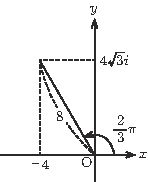
\includegraphics{./fig/sec00_3_1.pdf}}
$z^{3}=-4+4\sqrt{3}i$ ○○○○○○○ $z$ ○○○○○○○.
\begin{fleqn}[4zw]
\begin{alignat}{2}
&|-4+4\sqrt{3}i|=\sqrt{(-4)^{2}+(4\sqrt{3})^{2}}=8\notag\\
&\arg(-4+4\sqrt{3}i)=\frac{2}{3}\pi+2n\pi\notag
\end{alignat}
\end{fleqn}
○○○\hspace{1zw}$-4+4\sqrt{3}i=8\left (\cos\frac{2}{3}\pi+i\sin\frac{2}{3}\pi\right )$

$z=r(\cos\theta+i\sin\theta)\, (r>0,\ 0\leqq\theta<2\pi)$ ○○○○,○・○○○○○○○○○,
○○○○
\end{Mw}
\[
r^{3} (\cos 3\theta+i$ sin3 $\theta)=8\left(\cos\dfrac{2}{3}\pi+i\sin\dfrac{2}{3}\pi\right)
\]%
\settowidth{\dimen0}{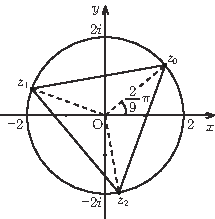
\includegraphics{./fig/0.pdf}}%
\begin{Mw}{\dimen0}{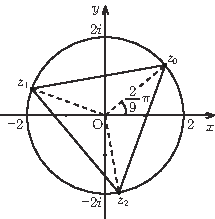
\includegraphics{./fig/0.pdf}}
○○○○○○○○○○○○○○○
\[
\hspace{1.5zw}r^{3}=8,\hspace{1zw}3\theta=\frac{2}{3}\pi+2n\pi\par
\]
\hspace{2zw}$\therefore \hspace{1zw} r=2,\hspace{1zw}\theta=\frac{2}{9}\pi+\frac{2n}{3}\pi$\\[3mm]
$ 0\leqq\theta<2\pi$ ○○ \hspace{1.5zw}$\theta=\frac{2}{9}\pi,\ \frac{2}{9}\pi+\frac{2}{3}\pi,\ \frac{2}{9}\pi+\frac{4}{3}\pi$
\begin{fleqn}
\begin{alignat}{3}
○○○\hspace{1zw}& z_{0}=2\left (\cos\frac{2}{9}\pi+i\sin\frac{2}{9}\pi\right ),&\notag\\[3mm]
&z_{1}=2\left (\cos\frac{8}{9}\pi+i\sin\frac{8}{9}\pi\right ),&\quad z_{2}=2\left (\cos\frac{14}{9}\pi+i\sin\frac{14}{9}\pi\right )\notag
\end{alignat}
\end{fleqn}

○○○○3○○○,○○○○○○○O(0) ○○○○○,○○ $\sqrt[3]{8}=2$ ○○○○3○○○○○ (○○2○○○○○○○○3○○○3○○) ○○○.○○○,
\end{Mw}

$\alpha=r_{0}(\cos\theta_{0}+i\sin\theta_{0})$ ○○○,①○○○○ $n$ ○○$z$○ $n$ ○○○
\begin{align*}
z_k&=\sqrt[n]{r_{0}}\left \{\cos\left (\frac{\theta_{0}}{n}+\frac{2k\pi}{n}\right )+i\sin\left (\frac{\theta_{0}}{n}+\frac{2k\pi}{n}\right )\right \}\\
&\phantom{=\;}\;(k=0,1,\ldots,n-1)
\end{align*}
○○○.○○○○○○,○ $z_{k}\, (k=0,1,\ldots,n-1)$ ○○O(0) ○○○○○,○○$\sqrt[n]{r_{0}}$ ○○○○ $n$ ○○○○○○○○.

\step{基本問題を解いてみよう}
\begin{例題}
○○○○○○○○○.\vs{-1.5mm}\par
\begin{longtable}[l]{@{}l@{\hskip4zw}l}
(1)\hspace{.5zw} $i$ ○○○○&(2) \hspace{.5zw}$-2+2\sqrt{3}i$ ○4○○
\end{longtable}\vs{-1.5mm}
\end{例題}

\begin{解答}
\vspace{-\baselineskip}\vspace{-\abovedisplayskip}
\begin{fleqn}[4zw]
\vspace{\baselineskip}\vspace{\abovedisplayskip}
(1)\hskip1zw$i=\cos\frac{\pi}{2}+i\sin\frac{\pi}{2}$\par
\noindent
$z^{2}=i$ ○○○○$z$○2○○○

\begin{alignat}{2}
z_k & =\cos\left(\frac{\pi}{4}+k\pi\right)+
i\sin\left(\frac{\pi}{4}+k\pi\right)\quad(k=0,1)\notag\\
z_{0}&=\cos\frac{\pi}{4}+i\sin\frac{\pi}{4}=\frac{1}{\sqrt{2}}(1+i)\notag\\[3mm]
z_{1}&=\cos\frac{5}{4}\pi+i\sin\frac{5}{4}\pi=-\frac{1}{\sqrt{2}}(1+i)\tag*{\kotae}
\end{alignat}
\end{fleqn}
\begin{fleqn}[4zw]
(2)\hspace{1zw} $-2+2\sqrt{3}i=4\left (\cos\frac{2}{3}\pi+i\sin\frac{2}{3}\pi\right )$\par\noindent
$z^{4}=-2+2\sqrt{3}i$ ○○○○$z$ ○4○○○
\end{fleqn}
\begin{fleqn}[1zw]
\begin{alignat*}{2}
z_{0}&=\sqrt[4]{4}\left (\cos\frac{1}{6}\pi+i\sin\frac{1}{6}\pi\right )=\sqrt{2}\left( \frac{\sqrt{3}}{2}+\frac{1}{2}i\right) = \frac{\sqrt{6}}{2}+\frac{\sqrt{2}}{2}i\\[3mm]
z_{1}&=\sqrt[4]{4}\left (\cos\frac{2}{3}\pi+i\sin\frac{2}{3}\pi\right )
=\sqrt{2}\left (-\frac{1}{2}+\frac{\sqrt{3}}{2}i\right )=-\frac{\sqrt{2}}{2}+\frac{\sqrt{6}}{2}i\\[3mm]
z_{2}&=\sqrt[4]{4}\left (\cos\frac{7}{6}\pi+i\sin\frac{7}{6}\pi\right )=\sqrt{2}\left( -\frac{\sqrt{3}}{2}-\frac{1}{2}i \right) =-\frac{\sqrt{6}}{2}-\frac{\sqrt{2}}{2}i \\[3mm]
z_{3}&=\sqrt[4]{4}\left (\cos\frac{5}{3}\pi+i\sin\frac{5}{3}\pi\right )
=\sqrt{2}\left (\frac{1}{2}-\frac{\sqrt{3}}{2}i\right )=\frac{\sqrt{2}}{2}-\frac{\sqrt{6}}{2}i\hspace{.5zw}{\kotae}
\end{alignat*}
\end{fleqn}
\end{解答}

\section{3○○○○○○○○○○}
\step{基本を確認しておこう}
○○○○,3○○○○ $a_{0}x^{3}+a_{1}x^{2}+a_{2}x+a_{3}=0\ (a_{0}\neq 0)$
\hfill{……①} \\
○○○○○○.○○○(○○○)○○○○○.
\setcounter{equation}{2}

①○○○○○○○○○○○○○○○○○.①○○○○ $a_{0}$ ○○○○
\[
x^{3}+ax^{2}+bx+c=0\ \left (a=\frac{a_{1}}{a_{0}},\hspace{1zw}b=\frac{a_{2}}{a_{0}},\hspace{1zw}c=\frac{a_{3}}{a_{0}}\right )
\]
○○○○○○,$x^{2}$ ○○○○○○○○○○,$x=y-\frac{a}{3}$ ○○○○,
\begin{align*}
\left (y-\frac{a}{3}\right )^{3}&+a\left (y-\frac{a}{3}\right )^{2}+b\left (y-\frac{a}{3}\right )+c=0\notag\\
\intertext{○○○○○○,
$p=-\frac{a^{2}}{3}+b,\ q=\frac{2}{27}a^{3}-\frac{ab}{3}+c$○○○○}
 y^{3}&+py+q=0\tag*{……②}
\end{align*}
○○○.○○○,$y=u+v$ ○○○○\hspace{2zw}$(u+v)^{3}+p(u+v)+q=0$
\[
u^{3}+v^{3}+q+(u+v)(3uv+p)=0
\]
{\mathindent0pt
\begin{empheq}[left=○○○○○\hspace{1zw}\empheqlbrace]{alignat=1}
&u^{3}+v^{3}+q=0 \\
&3uv+p=0
\end{empheq}}%\vspace{.25\baselineskip}

\noindent
○○○○ $u$ ○ $v$ ○○○○○○○○○○○○○,$y=u+v$ ○○ $y$, ○○○
$x=y-\frac{a}{3}$ ○○①○○ $x$ ○○○○○.○○○ $u, v$ ○③,④○○○○○○

\[
u^{3}+v^{3}=-q,\qquad u^{3}v^{3}=(uv)^{3}=\left (-\frac{p}{3}\right )^{3}=-\frac{p^{3}}{27}\]
○○○○○,$u^{3}$ ○ $v^{3}$ ○ $t$ ○2○○○○ $(t-u^{3})(t-v^{3})=0$ ○○,○○○○
\begin{fleqn}[4zw]
\begin{alignat}{1}
t^{2}+qt-\frac{p^{3}}{27}=0
\end{alignat}
\end{fleqn}
○○○○○○○○○.⑤○①○\textbf{○○○○○}○○○.○○,⑤○○○○
\begin{align*}
t=\frac{1}{2}\left (-q\pm\sqrt{q^{2}+\frac{4}{27}p^{3}}\right )=-\frac{q}{2}\pm\sqrt{\frac{q^{2}}{4}+\frac{p^{3}}{27}}
\end{align*}
○○○○○,$\frac{q^{2}}{4}+\frac{p^{3}}{27}=r$ ○○○○,$u^{3}=-\frac{q}{2}+\sqrt{r},\hspace{1zw}v^{3}=-\frac{q}{2}-\sqrt{r}$\par
\noindent
○○○,$u^{3}=A^{3}$ ($A$ ○○○) ○○○○
\begin{align*}
(u-A)(u^{2}+Au+A^{2})=0\hspace{1zw}○○,\ u=A, \frac{-1\pm\sqrt{3}i}{2}A
\end{align*}

$\frac{-1+\sqrt{3}i}{2}=\ruby{$\omega$}{○○○}$○○○○,\ $\omega^{2}=\left (\frac{-1+\sqrt{3}i}{2}\right )^{2}=\frac{-1-\sqrt{3}i}{2}$ ○○○○○ $u^{3}=A^{3}$ ○3○○ $u=A,\ \omega A,\ \omega^{2}A$ ○○○.


○○○○○,$1+\omega+\omega^{2}=0$ ○○○○○○ ③, ④○○○○ $u, v$ ○○○
\begin{alignat*}{2}
u&=\sqrt[3]{-\frac{q}{2}+\sqrt{r}}, & v&=\sqrt[3]{-\frac{q}{2}-\sqrt{r}}\\[3mm]
u&=\omega\sqrt[3]{-\frac{q}{2}+\sqrt{r}},& v&=\omega^{2}\sqrt[3]{-\frac{q}{2}-\sqrt{r}}\\[3mm]
u&=\omega^{2}\sqrt[3]{-\frac{q}{2}+\sqrt{r}},\qquad& v&=\omega\sqrt[3]{-\frac{q}{2}-\sqrt{r}}
\end{alignat*}
○3○○○○.○○○ $y=u+v$ ○○○○○○,○○○○○3○○ $y$, ○○○○②○3○
○○○○,①○3○○○○○○○.
\[\left\{
	\begin{array}{lll}
y_{1}&=\sqrt[3]{-\dfrac{q}{2}+\sqrt{r}}\ & +\;\sqrt[3]{-\dfrac{q}{2}-\sqrt{r}}\\[3mm]
y_{2}&=\omega\sqrt[3]{-\dfrac{q}{2}+\sqrt{r}}\ &+\;\omega^{2}\sqrt[3]{-\dfrac{q}{2}-\sqrt{r}}\\[3mm]
y_{3}&=\omega^{2}\sqrt[3]{-\dfrac{q}{2}+\sqrt{r}}\ &+\;\omega\sqrt[3]{-\dfrac{q}{2}-\sqrt{r}}
\end{array}\right.
\]
\pagebreak

\step{基本問題を解いてみよう}
\begin{例題}
○○3○○○○○○○.\par
\begin{longtable}[l]{l@{\hskip4zw}l}
(1)\hspace{1zw}$x^{3}+6x+2=0$ & (2)\hspace{1zw}$x^{3}+3x^{2}-3=0$
\end{longtable}
\end{例題}

\begin{解答}
%\vspace{-\baselineskip}\vspace{-\abovedisplayskip}
(1)\hspace{1zw}$\Mframe{x=u+v\text{○○○}}\Footnote{$x^2$○○○○○○○,○○○○$x=u+v$○○○○.}$○\vspace{-\abovedisplayskip}\par
\begin{fleqn}[4zw]
\begin{align*}
&(u+v)^{3}+6(u+v)+2=0\\
&u^{3}+v^{3}+2+(u+v)(3uv+6)=0\\
&\left\{\begin{array}{@{}l}
u^{3}+v^{3}+2=0\\
3uv+6=0
\end{array}\right.
\Longleftrightarrow
\left\{\begin{array}{@{}l}
u^{3}+v^{3}=-2\\
uv=-2
\end{array}\right.
\Longrightarrow
\left\{\begin{array}{@{}l}
u^{3}+v^{3}=-2\\
u^3v^3=(-2)^3=-8
\end{array}\right.
\end{align*}
○○○○ $u^{3}$ ○ $v^{3}$ ○ $t^{2}+2t-8=0$ ○2○○○○.
\[
(t-2)(t+4)=0$\hspace{1zw}○○,$t=2, -4
\]
○○○○○,1○○ $u, v$ ○
\[
u=\sqrt[3]{2},\ v=\sqrt[3]{-4}=-\sqrt[3]{4}
\]
○○○,○○○○ $x=x_{i}\,(i=1,2,3)$ ○
\begin{fleqn}[1zw]
\begin{align*}
&\left\{\begin{array}{l}
x_{1}=u+v=\sqrt[3]{2}-\sqrt[3]{4}\\
x_{2}=\omega u+\omega^{2}v=\sqrt[3]{2}\omega-\sqrt[3]{4}\omega^{2}\\
x_{3}=\omega^{2}u+\omega v=\sqrt[3]{2}\omega^{2}-\sqrt[3]{4}\omega
\end{array}\right. \left (\text{○○○,}\omega=\frac{-1+\sqrt{3}i}{2}\right )
\tag*{\Kotae}
\end{align*}
\end{fleqn}
(2)\hspace{1zw}$\Mframe{x=y-1\text{○○○}}\Footnote{$x^2$○○○○○○○○○,$x=y-1$○○○.}$○,$(y-1)^{3}+3(y-1)^{2}-3=0$
○○,$y^{3}-3y-1=0$\par
\noindent
$y=u+v$ ○○○○,$(u+v)^{3}-3(u+v)-1=0$
\[
u^{3}+v^{3}-1+(u+v)(3uv-3)=0
\]
\[
\left\{\begin{array}{@{}l}
u^{3}+v^{3}-1=0\\
3uv-3=0
\end{array}\right.
\Longleftrightarrow
\left\{\begin{array}{@{}r}
u^{3}+v^{3}=1\\
uv=1
\end{array}\right.
\Longrightarrow
\left\{\begin{array}{@{}r}
u^{3}+v^{3}=1\\
u^3v^3=1
\end{array}\right.
\]
○○○○ $u^{3}$ ○ $v^{3}$ ○,$t^{2}-t+1=0$ ○○○○
\begin{alignat}{2}
t&=\frac{1\pm\sqrt{3}i}{2}=\cos\left (\pm\frac{\pi}{3}\right )+i\sin\left (\pm\frac{\pi}{3}\right )\hspace{2zw}\text{(○○○○)}\notag\\
\intertext{○○○}
u^{3}&=\cos\frac{\pi}{3}+i\sin\frac{\pi}{3},\qquad
v^{3}=\cos\left (-\frac{\pi}{3}\right )+i\sin\left (-\frac{\pi}{3}\right )\notag
\end{alignat}
○○○○○○1○○ $u, v$ ○,○・○○○○○○○○○
\[
u=\cos\frac{\pi}{9}+i\sin\frac{\pi}{9},\ v=\cos\left (-\frac{\pi}{9}\right )+i\sin\left (-\frac{\pi}{9}\right )
\]
○○,○○○$y$○○○
\begin{align*}
y_{1}&=u+v=2\cos\frac{\pi}{9}\\
y_{2}&=\left (\cos\frac{2}{3}\pi+i\sin\frac{2}{3}\pi\right )\left (\cos\frac{\pi}{9}+i\sin\frac{\pi}{9}\right )\\
&\phantom{=\;} +\left\{\cos\left (-\frac{2}{3}\pi\right )+i\sin\left (-\frac{2}{3}\pi\right)\right\}\left\{\cos\left (-\frac{\pi}{9}\right )+i\sin\left (-\frac{\pi}{9}\right )\right\}\\
&=\cos\frac{7}{9}\pi+i\sin\frac{7}{9}\pi
+\cos\left (-\frac{7}{9}\pi\right )+i\sin\left (-\frac{7}{9}\pi\right )\\
&=2\cos\frac{7}{9}\pi
\end{align*}
○○○,$ y_{3}=\omega^{2}u+\omega v=2\cos\frac{13}{9}\pi$
\par\noindent
○○○,
\[
x_{1} = 2\cos\frac{\pi}{9} -1,\quad
x_{2} = 2\cos\frac{7}{9}\pi -1,\quad
x_{3} = 2\cos\frac{13}{9}\pi -1
\kotae\]
\end{fleqn}
\end{解答}

\section{○○○○}
\step{基本を確認しておこう}
2○○○○○○○○○○○○○○○○○○○○○○,○○○○○○○○○○.
\begin{titlebox}{○○○○}
\begin{fleqn}[4zw]
\begin{align*}
\sin(\alpha + \beta)=&\sin\alpha\cos\beta + \cos\alpha\sin\beta\tag*{……①}\\
\sin(\alpha - \beta)=&\sin\alpha\cos\beta - \cos\alpha\sin\beta\tag*{……②}\\
\cos(\alpha + \beta)=&\cos\alpha\cos\beta - \sin\alpha\sin\beta\tag*{……③}\\
\cos(\alpha - \beta)=&\cos\alpha\cos\beta + \sin\alpha\sin\beta\tag*{……④}\\
\tan(\alpha + \beta)=&\dfrac{\tan\alpha + \tan\beta}{1 - \tan\alpha\tan\beta}\tag*{……⑤}\\[3mm]
\tan(\alpha - \beta)=&\dfrac{\tan\alpha - \tan\beta}{1 + \tan\alpha\tan\beta}\tag*{……⑥}
\end{align*}
\end{fleqn}
\end{titlebox}

①,③,⑤○ $\alpha=\beta=\theta$ ○○○○,○○2○○○○○○○○○○.


\begin{titlebox}{2○○○○○}
\begin{fleqn}[4zw]
\[
\begin{array}{llr}
\sin 2\theta&= 2\sin\theta\cos\theta&\\[1mm]
\cos 2\theta&= \cos^2\theta - \sin^2\theta = 2\cos^2\theta - 1 
= 1-2\sin^2\theta\\
\tan2\theta&= \dfrac{2\tan\theta}{1-\tan^2\theta}&
\end{array}\tag*{……⑦}
\]
\end{fleqn}
\end{titlebox}

○○,$\tan\theta=m$ ○○○○○,○○○○○○○○○○○○○○○.
$$
\left\{\begin{array}{l}
\sin 2\theta=2\sin\theta\cos\theta=2\tan\theta\cdot\cos^{2}\theta=2\tan\theta\cdot\frac{1}{1+\tan^{2}\theta}=\frac{2m}{1+m^{2}}\\[3mm]
\cos 2\theta=2\cos^2\theta-1=2\cdot\frac{1}{1+\tan^{2}\theta}-1=\frac{1-m^{2}}{1+m^{2}}
\end{array}\right.
$$

○○○2○○○○○⑦○○,○○○○○○○○○○○○○○○○○.\\
$\cos 2\theta=2\cos^{2}\theta-1$ ○,$\theta$ ○○○○○ $\frac{\theta}{2}$ ○○○○
$\cos\theta=2\cos^{2}\frac{\theta}{2}-1\linebreak[4]\text{○○○,}\cos^{2}\frac{\theta}{2}=\frac{1+\cos\theta}{2}$

\begin{titlebox}{○○○○○}
\begin{fleqn}[1zw]
\[
\cos^2\frac{\theta}{2}=\frac{1+\cos\theta}{2},\qquad \sin^2\frac{\theta}{2}=\frac{1-\cos\theta}{2},\qquad
\tan^2\frac{\theta}{2}=\frac{1-\cos\theta}{1+\cos\theta}
\]
\end{fleqn}
\vspace{-3mm}
\end{titlebox}
\vspace{-3mm}
○○○,$ 3\theta=2\theta+\theta$ ○○○○,○○3○○○○○○○○○○.
\begin{titlebox}{3○○○○○}
\[\rule{0pt}{1.3zh}
\sin 3\theta=3\sin\theta-4\sin^3\theta,\qquad 
\cos 3\theta=4\cos^3\theta-3\cos\theta
\]\vspace{-3mm}
\end{titlebox}

%\begin{fleqn}[4zw]
\begin{fleqn}
\begin{align*}
\textbf{\fbox{例}}\qquad\sin3\theta&=\sin(2\theta+\theta)=\sin 2\theta\cos\theta+\cos 2\theta\sin\theta\notag\\
&=2\sin\theta\cos\theta\cdot\cos\theta+(1-2\sin^{2}\theta)\sin\theta\notag\\
&=2\sin\theta(1-\sin^{2}\theta)+\sin\theta-2\sin^{3}\theta=3\sin\theta-4\sin^{3}\theta\notag
\end{align*}
\end{fleqn}
○○,①$+$②,①$-$②,③$+$④,③$-$④ ○○○○○○○○○,○○○○○○.

\begin{titlebox}{○○○・○○○○○○}%
\setcounter{equation}{7}\hbox{}
\begin{fleqn}[3zw]
\begin{align}
\sin\alpha\cos\beta&=\phantom{-}\frac{1}{2}\{ \sin(\alpha+\beta) + \sin(\alpha-\beta)\} \\
\cos\alpha\sin\beta&=\phantom{-}\frac{1}{2}\{ \sin(\alpha+\beta) - \sin(\alpha-\beta)\}  \notag\\
\cos\alpha\cos\beta&=\phantom{-}\frac{1}{2}\{ \cos(\alpha+\beta) + \cos(\alpha-\beta)\}  \notag\\
\sin\alpha\sin\beta&=-\frac{1}{2}\{ \cos(\alpha+\beta) - \cos(\alpha-\beta)\}\notag
\end{align}
\end{fleqn}
\end{titlebox}
\begin{titlebox}{○・○○○○○○○○}
\hbox{}
\begin{fleqn}[3zw]
\begin{align}
\sin\alpha+\sin\beta&=\phantom{-}2\sin\frac{\alpha+\beta}{2}\cos\frac{\alpha-\beta}{2} \\
\sin\alpha-\sin\beta&=\phantom{-}2\cos\frac{\alpha+\beta}{2}\sin\frac{\alpha-\beta}{2}\notag\\
\cos\alpha+\cos\beta&=\phantom{-}2\cos\frac{\alpha+\beta}{2}\cos\frac{\alpha-\beta}{2}\notag\\
\cos\alpha-\cos\beta&=-2\sin\frac{\alpha+\beta}{2}\sin\frac{\alpha-\beta}{2}\notag
\end{align}
\end{fleqn}
\end{titlebox}

\begin{例}⑧○○ $\sin(A+B)+\sin(A-B)=2\sin A\cos B$
\end{例}

\noindent
$A+B=\alpha,  A-B=\beta$ ○○○○ $A=\frac{\alpha+\beta}{2}, B=\frac{\alpha-\beta}{2}$ ○○○,⑨ ○○○○○.

%\begin{Mw}{30mm}{\Fig{30mm}{24mm}}
\begin{Mw}{30mm}{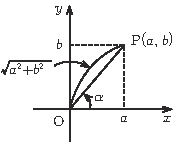
\includegraphics{./fig/sec00_5_1.pdf}}
○○○○ $ a\sin\theta+b\cos\theta$ ○,○ $\mathrm{P}(a,\ b)$ ○{\it xy}
○○○○○○○,$\mathrm{OP}=\sqrt{a^{2}+b^{2}}$ ○○○ $x$ ○○○○○○○
○ $\overrightarrow{\mathrm{OP}}=(a,\ b)$ ○○○○○○○○○ $\alpha$ ○○○○○○,
\end{Mw}
\begin{fleqn}[4zw]
\begin{alignat}{2}
&a\sin\theta+b\cos\theta\notag\\
=\;&\sqrt{a^2 + b^2}\left (\frac{a}{\sqrt{a^2 + b^2}}\sin\theta + \frac{b}{\sqrt{a^2 + b^2}}\cos\theta \right) \notag\\[3mm]
=\;&\sqrt{a^2 + b^2}(\cos\alpha\sin\theta + \sin\alpha\cos\theta) \notag\\[3mm]
=\;&\sqrt{a^2 + b^2}\sin(\theta + \alpha) \hspace{2zw} \left (\cos\alpha=\frac{a}{\sqrt{a^2 + b^2}}, \sin\alpha=\frac{b}{\sqrt{a^2 + b^2}} \right) \notag
\end{alignat}
\end{fleqn}

○○○○○,○○○○○\textbf{○○○○}○○○.

\step{基本問題を解いてみよう}

\begin{例題}[1]
$x, y$ \text{○○○○○○}
\begin{fleqn}[4zw]
\[
\left\{\begin{array}{rl}
13\,\cos x+\sqrt{3}\sin x&=y\cos x\\
\sqrt{3}\,\cos x+1\mathrm{l}\sin x&=y\sin x
\end{array}\right.
\]
\end{fleqn}
○2○○○○$(x_{1}, y_{1})$,\ $(x_{2}, y_{2})$(○○○,$0\leqq x_{1}\leqq x_{2}<\pi$)○○○○○,$x_{1}$, $y_{1}$, $x_{2}$, $y_{2}$○○○○○○.
\end{例題}
\vspace{\baselineskip}

\begin{解答}

\vspace{-\baselineskip}\vspace{-\abovedisplayskip}
\begin{fleqn}[4zw]
%\vspace{-\baselineskip}\vspace{-\abovedisplayskip}
\hspace{4zw}$\left\{\begin{array}{rrr}
13\,\cos x+\sqrt{3}\sin x&=y\cos x & \hspace{13zw}{……①}\\
\sqrt{3}\,\cos x+11\sin x&=y\sin x & \hspace{13zw}{……②}
\end{array}\right.$
\end{fleqn}

$\Mframe{\text{①}\times\sin x-\text{②}\times\cos x}$\Footnote{○○○○○○○○○$x,y$○○○,○○○○○○○○$y$○○○.}○○
\begin{fleqn}[4zw]
\begin{alignat*}{2}
&\sin x(13\cos x+\sqrt{3}\sin x)
-\cos x(\sqrt{3}\cos x+11\sin x)=0\notag\\
&\,2 \sin x\cos x- \sqrt{3}(\cos^{2}x-\sin^{2}x)=0\notag\\[-3pt]
&\sin 2x-\sqrt{3}\cos 2x=0\hspace{2zw}\therefore\hspace{1zw}\tan 2x=\frac{\sin 2x}{\cos 2x}=\sqrt{3}\notag
\end{alignat*}
\end{fleqn}

$ 0\leqq x<\pi$ ○○○ $ 0\leqq 2x<2\pi$ ○○○

\begin{fleqn}[4zw]
\begin{alignat*}{2}
&2x=\frac{\pi}{3},\ \frac{4}{3}\pi \qquad \therefore\quad x=\frac{\pi}{6},\ \frac{2}{3}\pi
\end{alignat*}
\end{fleqn}

①,②○○,$ 0\leqq x_{1}<x_{2}<\pi$ ○○○

\begin{fleqn}[4zw]
\begin{alignat*}{2}
&x_{1}=\frac{\pi}{6},\, y_{1}=14,\, x_{2}=\frac{2}{3}\pi,\, y_{2}=10 \tag*{\kotae}
\end{alignat*}
\end{fleqn}
%\vspace{\baselineskip}
\end{解答}

\begin{例題}[2]
○○ $x, y$ ○ $x^{2}+4xy+5y^{2}-3=0$ ○○○○○○○.○○○○,$2x^{2}+xy+3y^{2}$○○○○○○○○○○○○○.
\end{例題}

\medskip
\begin{解答}
$2x^{2}+xy+3y^{2}=P$ ○○○○
\begin{align*}
8x^{2}+4xy+12y^{2}\mathop{=}^{\text{\ajMaruKata{2}}}4P \tag*{……①}%\cdots\cdots\text{①}\\
\end{align*}
○○,○○○○
\[
x^{2}+4xy+5y^{2}=3\tag*{……②}
\]
○○○.① $-$ ②○○,$7x^{2}+7y^{2}=4P-3$,○○○○
\[
7(x^{2}+y^{2})=4P-3\tag*{……③}
\]
\addtocounter{footnote}{1}
\footnotetext{○○○$x^2+4\,xy+5y^2=3$○$xy$○○○4○○○○○,$4P$○○○○.}\footnotetext[3]{2○○○○○○○○○○○.}\footnotetext[4]{○○○○○○.}
○○○,○○○$(x,y)=(r\cos\theta,r\sin\theta)\ (r>0,\ 0\leqq\theta<2\pi)$
○○○○②○○○○○○○
\begin{fleqn}[4zw]
\begin{align}
(r\cos\theta)^{2}+4(r\cos\theta)(r\sin\theta)+5(r\sin\theta)^2=3\notag\\
(\cos^{2}\theta+4\sin\theta\cos\theta+5\sin^{2}\theta)r^{2}=3\notag
\end{align}
\end{fleqn}
○○○,
\begin{alignat}{2}
r^{2}&=\frac{3}{\cos^{2}\theta+4\sin\theta\cos\theta+5\sin^{2}\theta}\notag\\
&\qerel{=}{3}\frac{3}{{\displaystyle \frac{1+\cos 2\theta}{2}}+2\sin 2\theta+5\cdot{\displaystyle \frac{1-\cos 2\theta}{2}}}\notag\\
&=\frac{3}{3+2(\sin 2\theta-\cos 2\theta)}\qerel{=}{4}\frac{3}{3+2\sqrt{2}\sin{\displaystyle \left (2\theta-\frac{\pi}{4}\right )}}\notag
\end{alignat}

$ 0\leqq\theta<2\pi$ ○○○,$-1\leqq\sin\left (2\theta-\frac{\pi}{4}\right )\leqq 1$ ○○○

\begin{fleqn}[4zw]
\begin{alignat}{2}
&\frac{3}{3+2\sqrt{2}}\leqq r^{2}\leqq\frac{3}{3-2\sqrt{2}}\notag\\[3mm]
\therefore\hspace{1zw} &3 (3-2\sqrt{2})\leqq r^{2}\leqq 3(3+2\sqrt{2})\tag*{……④}
\end{alignat}
\end{fleqn}

③○○,$7r^{2}=4P-3$ ○○○,\hspace{2zw}$P=\frac{7r^{2}+3}{4}$

○○○,④○○
\[
\frac{3(11-7\sqrt{2})}{2}\leqq P\leqq\frac{3(11+7\sqrt{2})}{2}\tag*{\kotae}
\]
%%%%%%%%○○○○○○、2Q○○○○○○○%%%%%%%%
\setcounter{footnote}{4}
{\footnotesize
\textbf{\fbox{○○}}\quad ○○○$\mathrm{C}_1: \, x^2+4xy+5y^2-3=0$○,
○○○○○○○○$\mathrm{C}_2: \, 2x^2+xy+3y^2=P$○○○○○$x, \, y$○○○○○2○○○○○,
○○○○○○○○$(x, \, y)$○○○○○○\Mframe{2○○○}\footnote{2○○○○○○○○,○○○『○○○○! ○○○○1○1○ ○○○○』○○○○○○.○○○○2○○○○○○○○○○○○○○○○○.}○○○.
2○○○○○○○○○○○○○○○○○○,○○○$\mathrm{C}_1, \, \mathrm{C}_2$○○○○○○○○○○○○○○○○.
○○○○○$\mathrm{C}_2$○$P$○○○○○○○,○○○○$P=5, 10$○○○○○○○○○○.
(○○○○○○○○○○○○,)$P$○○○○○○○○○$C_2$○○○○○○.

 ○○○○○,○$(x, \, y)$○○○○○○○○○○○○○○○○,$P$○○○○○○○○○○○○○○○○○○○○○○○○.
○○○○○○,
○○$\mathrm{C}_1$○○○$\mathrm{C}_2$○○○○○○○○○○○○○○$P$○○○○○○○○○○○○○○○○○○○○○○○○○○○.
○○○○○○$P$○○○○○○○○○○○,○○○○○○○○○$\mathrm{C}_2$○○○$\mathrm{C}_1$○○○,○○○○○○○○○○○○○.\VS{.5}
\begin{center}
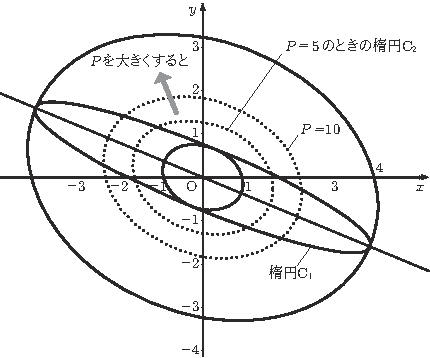
\includegraphics[scale=1]{./fig/sec00_betsu02.pdf}
\end{center}

\VS{.5}
○○,\hspace{1zw}$P=\frac{3(11\pm 7\sqrt{2})}{2}$ ○○○
\[
r^{2}=3(3\pm 2\sqrt{2}) \quad  \text{○○} \quad  \sin\left(2\theta-\frac{\pi}{4}\right)=\mp 1\quad \text{(○○○○)}
\]\par}
%%%%%%%%%%%%%%%%%%%%%%%%%%%%%%%%%%%%%%%%%%%%%%
\end{解答}
\section{○○○(1)}

\step{基本を確認しておこう}

○○ $\{a_{n}\}$ ○○○○○○○○○○○○○○○○○○○○○○○○○○○○○○,\textbf{○○○○○○○○}○○○,○○○○○○○○○\textbf{○○○}○○○.

\begin{titlebox}{○○○○,○○○○○○○○○○}
\vskip1mm

\hspace{4zw}
$\begin{array}{l}
\text{○○○○:\ } a_{n+1}-a_n=d\hspace{1zw}(n \geqq 1,\ d\text{○○○})\\
\text{○○○○:\ } a_{n+1}=ra_n\hspace{1zw}(n \geqq 1,\ r\text{○○○})
\end{array}$\\
\vskip-.5mm
\end{titlebox}

○○○○○(○○○)○○○○,○○○○○○○○○○○○○○.○○○○○○○○○○.

\begin{titlebox}{2○○○○○○}
\vskip1mm
a.\hspace{1zw}
$a_{n+1}=a_n+f(n)\hspace{1zw}(n \geqq 1)\qquad(\text{○○○})$
\end{titlebox}
 ○○○○ $n$ ○$1, 2, \ldots, n-1$ ○○○○○,○々○○○○
\[
a_{n}=a_{\mathrm{1}}+\sum_{k=1}^{n-1}f(k)\hspace{1zw}(n\geqq 2)
\]

\begin{shadebox}
b.\hspace{1zw}$a_{n+1}=pa_n+q\hspace{2zw}(n \geqq 1,\ p \neq 0,1,\ q \neq 0)$
\end{shadebox}
 $a_{n},\ a_{n+1}$ ○ $t$ ○○○○, $\Mframe{t=pt+q}$\Footnote{○○○○○○○○○○○.} ○○○○, $t=\frac{q}{1-p}$

\noindent
○○ $t$ ○○○○○○○○○○○○○○\hspace{1zw} $a_{n+1}-\frac{q}{1-p}=p\left (a_{n}-\frac{q}{1-p}\right )$\par
\noindent
$a_{n}-\frac{q}{1-p}=\left (a_{1}-\frac{q}{1-p}\right )p^{n-1}\hspace{2zw}\therefore\hspace{1zw}a_{n}=\frac{q}{1-p}+\left (a_{1}-\frac{q}{1-p}\right )p^{n-1}$
\begin{shadebox}
c.\hspace{1zw}$a_{n+1}=pa_n+f{(n)}\hspace{2zw}(n \geqq 1,\ p \neq 0,1)$
\end{shadebox}
 ○○○ $p^{n+1}$ ○○○○ 

\[
\frac{a_{n+1}}{p^{n+1}}=\frac{a_{n}}{p^{n}}+\frac{f(n)}{p^{n+1}}=\frac{a_{n}}{p^{n}}+g(n)$\hspace{2zw}$\bigg (g(n)=\dfrac{f(n)}{p^{n+1}}$ ○○○ $\bigg )
\]

$\frac{a_{n}}{p^{n}}=b_{n}$ ○○○○ $b_{n+1}=b_{n}+g(n)$ ○○○,○○○a.○○○○○.\begin{shadebox}
d.\hspace{1zw}$a_{n+1}=\dfrac{pa_{n}+q}{ra_{n}+s} \quad (n \ge1, \, q \neq 0, \, r\neq 0, \, ps-qr\neq 0)$
\end{shadebox}
 $a_{n},a_{n+1}$○$t$○○○○,$t=\dfrac{pt+q}{rt+s}$ ○○○.
○○○○○$t$○○○○○2○○○○$rt^{2}+(s-p)t-q=0 \, (r \neq 0)$○○○,○○○○○○○○2○○○○$\alpha, \beta$○○○.

\noindent
(i) $\alpha \neq \beta$○○○;

○○○○○○○○$\alpha$○○○○
\[
a_{n+1}-\alpha
=\dfrac{pa_{n}+q}{ra_{n}+s}-\alpha=\frac{(p-r\alpha)a_{n}+q-s\alpha}{ra_{n}+s}
\]
$r\alpha^{2}+(s-p)\alpha-q=0$○○$q-s\alpha=-\alpha(p-r\alpha)$○○○○○
\begin{align}
a_{n+1}-\alpha
&=\dfrac{(p-r\alpha)(a_{n}-\alpha)}{ra_{n}+s} \\
\intertext{○○○,}
a_{n+1}-\beta
&=\dfrac{(p-r\beta)(a_{n}-\beta)}{ra_{n}+s}
\end{align}

①$\div$②○○
$\dfrac{a_{n+1}-\alpha}{a_{n+1}-\beta}
=\dfrac{p-r\alpha}{p-r\beta} \cdot \dfrac{a_{n}-\alpha}{a_{n}-\beta}$

○○○○○,$\dfrac{a_{n}-\alpha}{a_{n}-\beta}=b_{n}$○○○○,
$b_{n+1}=\dfrac{p-r\alpha}{p-r\beta}b_{n}$○○○,○○$\{ b_{n} \}$○○○○○○○○.
○○○○○○○○○○○,$\{ a_{n} \}$○○○○○○○○○.

\noindent
(ii) 
$\alpha=\beta$○○○;

①,②○○○○○.
①○○○○○○○○○○$\dfrac{1}{a_{n}-\alpha}=c_{n}$○○○○○○○○,○○$\{ c_{n} \}$○○○○○○○○○.

\step{基本問題を解いてみよう}
\begin{例題}
○○ $\{a_{n}\}$ ○○○○,○○○○○○○○○,○○○○○○○○○○○○.

\begin{Description}{2.5zw}
\item[(1)]
$a_{1}=2,\ a_{n}=a_{n-1}+n(n-1)\quad (n\geqq 2)$
\item[(2)]
$a_{1}=2,\ a_{n+1}=\frac{a_{n}}{a_{n}+3}\quad (n \geqq 1)$
\item[(3)]
$a_{1}=2,\ a_{n+1}=\frac{a_{n}+2}{2a_{n}+1}\quad (n\geqq 1)$
\end{Description}
\end{例題}

\begin{解答}
(1) ○○○○○ $a_{n+1}-a_{n}=n(n+1)$ ○,$n\geqq 2$ ○○○\footnotetext[2]{$a_n-a_{n-1}=n(n-1)$○○$a_n=a_1+\sum_{k=1}^{n-1}k(k-1)$○○○○○○○○.}
\begin{align*}
%& \Mframe{a_{n}=a_{1}+\sum_{k=1}^{n-1}k(k+1)}\Footnotemark[2] \qerel{=}{2}2+\frac{1}{3}(n-1)n(n+1)\\
& \Mframe{a_{n}=a_{1}+\sum_{k=1}^{n-1}k(k+1)}\Footnotemark[2] \mathop{=}^{\text{\ajMaruKata{3}}}2+\frac{1}{3}(n-1)n(n+1)\\
&\hphantom{a=}=\frac{n^{3}-n+6}{3}=\frac{1}{3}(n+2)(n^{2}-2n+3)
\end{align*}
$a_{1}=2$ ○○○,○○○○ $n=1$ ○○○○○○.○○○,\footnotetext[3]{$\sum_{k=1}^{n}k(k+1)=\frac{1}{3}n(n+1)(n+2)$○○○○.}
\begin{equation*}
a_{n}=\frac{1}{3}(n+2)(n^{2}-2n+3)\tag*{\kotae}
\end{equation*}

(2) ○○○○○○○○○○○○○
\begin{align*}
\frac{1}{a_{n+1}}=\frac{a_{n}+3}{a_{n}}=1+\frac{3}{a_{n}}
\end{align*}
$\frac{1}{a_{n}}=b_{n}$ ○○○○\hspace{1zw}$b_{n+1}=3b_{n}+1$\vs{-2mm}
\begin{align*}
\Mframe{b_{n+1}+\frac{1}{2}=3\left (b_{n}+\frac{1}{2}\right )}\Footnotemark[4]
\end{align*}\footnotetext[4]{○○○○○$t=3t+1$○○○○$t=-\frac{1}{2}$}
○○○○○,○○ $\left\{b_{n}+\frac{1}{2}\right\}$ ○○○ $b_{1}+\frac{1}{2}=\frac{1}{a_{1}}+\frac{1}{2}=1$,
○○○3○○○○○○○○
\[
b_{n}+\frac{1}{2}=1\cdot 3^{n-1} \hspace{3zw} \therefore \hspace{1zw} b_{n}=\frac{2\cdot 3^{n-1}-1}{2}
\]
\begin{fleqn}
\begin{alignat}{1}
\text{○○○,}\hspace{.5zw}a_{n}=\frac{1}{b_{n}}=\frac{2}{2\cdot 3^{n-1}-1}\tag*{\kotae}
\end{alignat}
\end{fleqn}

(3)\ ○○○○○ $t=\dfrac{t+2}{2t+1}$○○○○,$t^{2}=1$○○$t=\pm1$.
○○○○
\begin{fleqn}[4zw]
\begin{alignat}{3}
&a_{n+1}-1&\;=\frac{a_{n}+2}{2a_{n}+1}-1=-\frac{a_{n}-1}{2a_{n}+1}\notag\\[3mm]
&a_{n+1}+1&\;=\frac{a_{n}+2}{2a_{n}+1}+1=\frac{3(a_{n}+1)}{2a_{n}+1}\notag
\end{alignat}
\end{fleqn}
\text{○○○○○,}\ $\frac{a_{n+1}-1}{a_{n+1}+1}=-\frac{1}{3}\cdot\frac{a_{n}-1}{a_{n}+1}$

$b_{n}=\frac{a_{n}-1}{a_{n}+1}$ ○○○○\hspace{.5zw} $b_{n+1}=-\frac{1}{3}b_{n}$

$b_{1}=\frac{a_{1}-1}{a_{1}+1}=\frac{1}{3}$ ○○\hspace{.5zw} $b_{n}=\frac{1}{3}\left (-\frac{1}{3}\right )^{n-1}=-\left (-\frac{1}{3}\right )^{n}$

\begin{fleqn}
\begin{alignat}{1}
○○○,a_{n}\qerel{=}{5}\frac{1+b_{n}}{1-b_{n}}=\frac{1-\left (-\frac{1}{3}\right )^{n}}{1+\left (-\frac{1}{3}\right )^{n}}=\frac{3^{n}-\left (-1\right )^{n}}{3^{n}+(-1)^{n}}\tag*{\kotae}
\end{alignat}\footnotetext[5]{$(a_n+1)b_n=a_n-1$○$a_n$○○○○○○○○.}
\end{fleqn}


\end{解答}

\section{○○○(2)}
\step{基本を確認しておこう}

\begin{titlebox}{3○○○○○○}
$\hspace{4zw}a_{n+2}=pa_{n+1}+qa_{n}\, (p\neq 0,\ q\neq 0)$
\end{titlebox}
○○○○ $a_{n+2},\ a_{n+1},\ a_n$○○○○○ $t^{2}, t, 1$○○○○○○ $t$ ○2○○○○ $t^{2}-pt-q=0$○○○○.○○○○○○○○2○○ $\alpha,\ \beta$ ○○○○,○○○○○○○○○
$
\alpha+\beta=p,\ \alpha\beta=-q
$○○○,○○○ $a_{n}$ ○○○○○○○○○○○○.

\begin{fleqn}[4zw]
\[
\begin{array}{r@{\ }l}
\text{(i)}&\alpha\neq\beta\text{○○○,\null}a_{n}=A\cdot\alpha^{n-1}+B\cdot\beta^{n-1}\\[1mm]
\text{(ii)}&\alpha=\beta\text{○○○,\null}a_{n}=(An+B)\cdot\alpha^{n-1}
\end{array}(A,\ B\ \text{○○○})
\]
\end{fleqn}

\begin{zDescription}
\item[\hbox{(i)}] $\alpha\neq\beta$ ○○○
\begin{align*}
a_{n+2}-\alpha a_{n+1}&=pa_{n+1}+qa_{n}-\alpha a_{n+1}=(p-\alpha)a_{n+1}+qa_{n}\\
&=\beta a_{n+1}-\alpha\beta a_{n}=\beta(a_{n+1}-\alpha a_{n})
\end{align*}
\begin{fleqn}[0zw]
\begin{alignat}{2}
\text{○○○○,}\ & a_{n+1}-\alpha a_{n}=(a_{2}-\alpha a_{1})\beta^{n-1}\tag*{……①}\\%
\mbox{○○○,}\hspace{1.3zw} & a_{n+1}-\beta a_{n}=(a_{2}-\beta a_{1})\alpha^{n-1}\tag*{……②}
\end{alignat}
\end{fleqn}
$\text{①}-\text{②}$○○,$(\beta-\alpha)a_{n}=(a_{2}-\alpha a_{1})\beta^{n-1}-(a_{2}-\beta a_{1})\alpha^{n-1}$\\
○○○,$a_{n}=\frac{1}{\beta-\alpha}\{(a_{2}-\alpha a_{1})\beta^{n-1}-(a_{2}-\beta a_{1})\alpha^{n-1}\}$

\item[\hbox{(ii)}]
$ \alpha=\beta$ ○○○\par
①,②○○○○,$a_{n+1}-\alpha a_{n}=(a_{2}-\alpha a_{1})\alpha^{n-1}$ ○○○○○,○○○ $\alpha^{n+1} (\neq 0)$ ○○○○○○○○ $a_{n}$ ○○○○○○○○○○.
\end{zDescription}

\begin{titlebox}{○○○○○}
\[\left\{\begin{array}{l}
a_{n+1}=pa_{n}+qb_{n}\\
b_{n+1}=ra_{n}+sb_{n}
\end{array}\right.\]
\end{titlebox}
$\{a_{n}\}$ ○○○○○○○3○○○○○○○○○○,○○○○○○○.

\begin{fleqn}[4zw]
\begin{alignat}{2}
a_{n+2}&=pa_{n+1}+qb_{n+1}=pa_{n+1}+q(ra_{n}+sb_{n})\notag\\
&=pa_{n+1}+qra_{n}+s(a_{n+1}-pa_{n})=(p+s)a_{n+1}-(ps-qr)a_{n}\notag
\end{alignat}
\end{fleqn}
○○○○,○○ $\{a_{n}+\alpha b_{n}\}$ ○○○ $\beta$ ○○○○○○○○○○○○○○○○○.

\noindent
$a_{n+1}+\alpha b_{n+1}=\beta(a_{n}+\alpha b_{n}) \text{○○}$
\begin{fleqn}[4zw]
\begin{alignat}{2}
(pa_{n}+qb_{n})+\alpha(ra_{n}+sb_{n})&=\beta(a_{n}+\alpha b_{n})\notag\\
(p+\alpha r)a_{n}+(q+\alpha s)b_{n}&=\beta a_{n}+\alpha\beta b_{n}\notag
\end{alignat}
\end{fleqn}
○○○○,$ p+\alpha r=\beta$ ○○ $ q+\alpha s=\alpha\beta$ ○○ $\alpha, \beta$ ○○○○○○.

\step{基本問題を解いてみよう}

\begin{例題}
%\vspace{-\baselineskip}\vspace{-\abovedisplayskip}
\begin{fleqn}[4zw]
(1)\ ○○ $\{a_{n}\}$ ○ $a_{n+2}=4a_{n+1}-4a_{n}\,(n\geqq 1) , a_{1}=1, a_{2}=8$○○○○○○○○,○○○ $a_{n}$ ○○○○.\par
\noindent
(2)\ 2○○○○ $\{x_{n}\}, \{y_{n}\}$ ○○○○
\[
x_{1}=11,\quad y_{1}=1,\quad x_{n+1}=6x_{n}+5y_{n},\quad y_{n+1}=x_{n}+2y_{n}\,(n\geqq 1)
\]
○○○○○○○○,○○○ $x_{n}, y_{n}$ ○○○○.
\end{fleqn}
\end{例題}

\medskip
\begin{解答}
%\vspace{-\baselineskip}\vspace{-\abovedisplayskip}
(1)\ ○○○○○$t^{2}-4t+4=0$ ○○○○,$(t-2)^{2}=0$○○
$t=2$(2 \text{○○}).

\begin{fleqn}[4zw]
○○○○,$a_{n+2}-2a_{n+1}=2(a_{n+1}-2a_{n})$

○○○○○,○○ $\{a_{n+1}-2a_{n}\}$ ○○○ $a_{2}-2a_{1}=8-2\cdot 1=6$,○○2○○○○○○○○
\begin{align*}
a_{n+1}-2a_{n}=6\cdot 2^{n-1}=3\cdot 2^{n}
\end{align*}
○○○ $2^{n+1}$ ○○○○
$\Mframe{\frac{a_{n+1}}{2^{n+1}}-\frac{a_{n}}{2^{n}}=\frac{3}{2}}
\Footnote{$\frac{a_n}{2^n}=b_n$○○○○$b_{n+1}-b_{n}=\frac{3}{2}$(=○○)}$\\
○○ $\left\{\frac{a_{n}}{2^{n}}\right\}$ ○○○ $\frac{a_{1}}{2^{1}}=\frac{1}{2}$,○○ $\frac{3}{2}$ ○○○○○○○○,
\[
\frac{a_{n}}{2^{n}}=\frac{1}{2}+(n-1)\cdot\frac{3}{2}=\frac{3n-2}{2}
\]

\end{fleqn}
\begin{fleqn}

\noindent
\begin{align*}
\text{○○○,}\hspace{.5zw}a_{n}=(3n-2)\cdot 2^{n-1}\tag*{\kotae}
\end{align*}

\end{fleqn}
\begin{fleqn}[4zw]

(2) \hspace{1zw} $x_{n+1}=6x_{n}+5y_{n},y_{n+1}=x_{n}+2y_{n}$

$y_n$○○○○○ $x_{n}$ ○○○○○○○○○○
\begin{alignat}{2}
x_{n+2}&=6x_{n+1}+5y_{n+1}=6x_{n+1}+5(x_{n}+2y_{n})\notag\\
&=6x_{n+1}+5x_{n}+2(x_{n+1}-6x_{n})=8x_{n+1}-7x_{n}\notag
\end{alignat}
○○○○,$x_{n+2}=8x_{n+1}-7x_{n}$\\
○○○○○$t^2=8t-7$○○○○,$t=1,7$

○○○○○○○○○○○,
\begin{alignat}{3}
& x_{n+2}-x_{n+1}&&=7(x_{n+1}-x_{n})\tag*{……①}\\
& x_{n+2}-7x_{n+1}&&=x_{n+1}-7x_{n}\tag*{……②}
\end{alignat}
\end{fleqn}
\begin{fleqn}[4zw]
①○○,○○ $\{x_{n+1}-x_{n}\}$ ○○○ $x_{2}-x_{1}=71-11=60$,○○7○○○○○○○○
\begin{alignat*}{1}
x_{n+1}-x_{n}=60\cdot 7^{n-1}\tag*{……③}
\end{alignat*}
②○○,○○ $\{x_{n+1}-7x_{n}\}$ ○○○ $x_{2}-7x_{1}=71-77=-6$ ○○○○○○○○
\begin{alignat*}{1}
x_{n+1}-7x_{n}=-6 \tag*{……④}
\end{alignat*}
$\text{③}-\text{④}$○○ $6x_{n}=60\cdot 7^{n-1}+6$.○○○,
$x_{n}=10\cdot 7^{n-1}+1 $

○○○○○
\begin{alignat*}{1}
5y_{n}&=x_{n+1}-6x_{n}\notag\\
&=(10\cdot 7^{n}+1)-6(10\cdot 7^{n-1}+1)=10\cdot 7^{n-1}-5\notag
\end{alignat*}

○○○,$y_{n}=2\cdot 7^{n-1}-1$

○○○○,
\[
x_n=10\cdot7^{n-1}+1,\qquad y_n=2\cdot7^{n-1}-1\tag*{\kotae}
\]
\end{fleqn}
\end{解答}

\section{○○○○}
\step{基本を確認しておこう}


\begin{titlebox}{○○○○}
○○○○○○ $n$ ○○○○,
\begin{fleqn}[1zw]
\begin{alignat*}{2}
(a+b)^n &= \sum_{r=0}^{n}\,{}_{n}\!\mathrm{C}_{r}a^{n-r}b^r\\
&={}_{n}\!\mathrm{C}_{0}a^n+{}_{n}\!\mathrm{C}_{1}a^{n-1}b+\cdots
+{}_{n}\!\mathrm{C}_{r}a^{n-r}b^r+\cdots+{}_{n}\!\mathrm{C}_{n}b^n\notag
\end{alignat*}
\end{fleqn}
\end{titlebox}

○○○○○○○○○${}_{n}\!\mathrm{C}_{r}\,(r=0,1,2,\ldots,\ n)$ ○○○○○○○○.${}_{n}\!\mathrm{C}_{r}$○$\Binom{n}{r}$○○○○○○○○.○○○ $n$ ○○○○○○ $r$ ○○○○○○○○○○○○○.○○,○○○○○○○ $(r+1)$ ○○○○ ${}_{n}\!\mathrm{C}_{r}a^{n-r}b^{r}$ ○,$(a+b)^{n}$ ○○○○○\textbf{○○○}○○○.○○,
\begin{fleqn}[2zw]
\begin{equation}
(1+x)^{n}=\sum_{r=0}^{n}{}_{n}\!\mathrm{C}_{r}x^{r}={}_{n}\!\mathrm{C}_{0}+{}_{n}\!\mathrm{C}_{1}x+{}_{n}\!\mathrm{C}_{2}x^{2}+\cdots+{}_{n}\!\mathrm{C}_{n}x^{n}\tag*{……①}
\end{equation}
\end{fleqn}

\noindent
○○○,○○○○○○○○○○○○○○○○○○○.\par
\noindent
$x=1$ ○○○○ ${}_{n}\!\mathrm{C}_{0}+{}_{n}\!\mathrm{C}_{1}+{}_{n}\!\mathrm{C}_{2}+\cdots+{}_{n}\!\mathrm{C}_{n}=2^{n}$\par
\noindent
$x=-1$ ○○○○ ${}_{n}\!\mathrm{C}_{0}-{}_{n}\!\mathrm{C}_{1}+{}_{n}\!\mathrm{C}_{2}-\cdots+(-1)^{n}{}_{n}\!\mathrm{C}_{n}=0$

\noindent
①○○○○ $x$ ○○○○○
\begin{fleqn}[4zw]
\begin{alignat*}{1}
n(1+x)^{n-1}={}_{n}\!\mathrm{C}_{1}+2 {}_{n}\!\mathrm{C}_2x+3{}_{n}\!\mathrm{C}_{3}x^{2}+\cdots+n{}_{n}\!\mathrm{C}_{n}x^{n-1}
\end{alignat*}
\end{fleqn}\par
\noindent
$x=1$ ○○○○ ${}_{n}\!\mathrm{C}_{1}+2{}_{n}\!\mathrm{C}_{2}+3{}_{n}\!\mathrm{C}_{3}+ \cdots +n_{n}\!\mathrm{C}_{n}=n\cdot 2^{n-1}$

\step{基本問題を解いてみよう}
\begin{例題}
(1) \quad $\frac{1\cdot {}_{10}\mathrm{C}_{1}+2\cdot {}_{10}\mathrm{C}_{2}+3\cdot {}_{10}\mathrm{C}_{3}+\cdots+10\cdot {}_{10}\mathrm{C}_{10}}{{}_{10}\mathrm{C}_{0}+{}_{10}\mathrm{C}_{1}+{}_{10}\mathrm{C}_{2}+\cdots+_{10}\!\mathrm{C}_{10}}$ ○○○○○○.
(2) \quad $\sum_{k=1}^{n}(x+2)^{k}$ ○○○○○○○○ $x$ ○○○○○○○.
\end{例題}

\begin{解答}
(1) \hspace{.5zw} $k$ ○○○○○○○

\begin{fleqn}[4zw]
\[
k\cdot {}_{10}\mathrm{C}_{k}=k\cdot\frac{10!}{k!(10-k)!}
=\frac{10\cdot 9!}{(k-1)!\{9-(k-1)\}!}=10\cdot {}_{9}\mathrm{C}_{k-1}
\]
\begin{alignat*}{2}
\text{○○} &=\sum_{k=1}^{10}k\cdot_{10}\mathrm{C}_{k}=\sum_{k=1}^{10}10\cdot {}_{9}\mathrm{C}_{k-1}\notag\\[3mm]
&=10({}_{9}\mathrm{C}_{0}+{}_{9}\mathrm{C}_{1}+{}_{9}\mathrm{C}_{2}+\cdots+{}_{9}\mathrm{C}_{9})\notag\\
&=10(1+1)^{9}=10\cdot 2^{9}=5\cdot 2^{10}
\end{alignat*}
$\text{○○,○○} =(1+1)^{10}=2^{10}$\\
$\text{○○○,○○} =\frac{5\cdot 2^{10}}{2^{10}}=5$\hfill{\kotae}

\noindent
(2)\hspace{1zw}$(x+2)^{k}={}_{k}\mathrm{C}_{0}\cdot 2^{k}+{}_{k}\mathrm{C}_{1}\cdot 2^{k-1}x+{}_{k}\mathrm{C}_{2}\cdot 2^{k-2}x^{2}+\cdots+_{k}\!\mathrm{C}_{k}x^{k}$
\end{fleqn}

\hspace*{1zw}%
$\sum_{k=1}^{n}(x+2)^{k}$ ○○○○○○○○ $x$ ○○○○,
\begin{fleqn}[4zw]
\[
\sum_{k=1}^{n}{}_{k}\mathrm{C}_{1}\cdot 2^{k-1}=\sum_{k=1}^{n} k\cdot 2^{k-1}\,(\Mframe{=S_n○○○}\Footnotemark[1])
\]
\addtocounter{footnote}{1}
\footnotetext[1]{$S_{n}= \displaystyle \sum_{k=1}^{n} k \cdot r^{k-1} \, (r \neq 0, \, 1)$○$S_{n}-rS_{n}$○○○○○○○○○○○○.
}
\end{fleqn}

%%%%%%○○○○○%%%%%%
%\hspace*{1zw}%
%$k\cdot 2^{k-1}=(k-1)\cdot 2^{k}-(k-2)\cdot 2^{k-1}$ ○○○
%\begin{fleqn}[4zw]
%\begin{alignat*}{2}
%S_{n}&=\sum_{k=1}^{n}\{(k-1)\cdot 2^{k}-(k-2)\cdot 2^{k-1}\}\notag\\[3mm]
%&=(n-1)\cdot 2^{n}+1\tag*{\kotae}
%\end{alignat*}
%\end{fleqn}

\begin{center}
$
\begin{array}{lcllrl}
 S_{n}&=&1+2 \cdot & 2+3 \cdot 2^{2}+\cdots &+n     \cdot 2^{n-1}& \\
2S_{n}&=&          & 2+2 \cdot 2^{2}+\cdots &+(n-1) \cdot 2^{n-1}& +n \cdot 2^{n}
\end{array}$
\end{center}
○々○○○○,
\begin{align*}
-S_{n}&=1+2+2^{2}+\cdots+2^{n-1}-n \cdot 2^{n} \\
      &=\dfrac{2^{n}-1}{2-1}-n \cdot 2^{n}
       =-(n-1) \cdot 2^{n}-1
\end{align*}
○○○,○○○$x$○○○○
\[
S_{n}=(n-1)\cdot2^{n}+1 \hfill\text{……(○)}
\]
\end{解答}
\step{○○○○○○○○○○!}
\begin{問題}[1]
 ○○○○○○○○○○○○○○○○○○○○.
\[
\left\{\begin{array}{l}
 x^{3}+xy+y^{3}=11 \\ 
 x^{3}-xy+y^{3}=7
\end{array}\right.
\]
\end{問題}
\begin{解答}
\[
\left\{\begin{array}{l}
 x^{3}+xy+y^{3}=11 \\ 
 x^{3}-xy+y^{3}=7
 \end{array}\right.
	\tag*{$\begin{array}{r@{}}
	{……①}\\
	{……②}\end{array}$%
	}%
\]
○○○.

①+②○○${2}x^{3}+2y^{3}=18$,○○○○$x^{3}+y^{3}=9$\,\hfill{……③}

(①-②)$\div 2$○○$xy=2$,○○○○$x^{3}y^{3}=8$\,\hfill{……④}

③,④○○$x^{3},\,y^{3}\!$○○○○○2○○○○○${t}^{2}-9t+8=0$

○○○○○○ $t=1,8$

○○○$(x^{3},y^{3})=(1,8)$,$(8,1)$

$(x^{3},y^{3})=(1,8)$○○○,○○○○○ $x^{3}=1,\, xy=2$ ○○○○
\[
(x,y)=(1,2),\left( \frac{-1\pm \sqrt 3 
i}{2},-1\mp \sqrt 3 i \right)\qquad\text{(○○○○)}
\]

$(x^{3},y^{3})=(8,1)$○○○,○○○○○ $x^{3}=8,\, xy=2$ ○○○○
\[
(x,y)=(2,1),\left( -1\pm \sqrt{3}i,\frac{-1\mp 
\sqrt{3} i}{2} \right)\qquad\text{(○○○○)}
\]
 
○○○○

$
(x,y)=(1,2),(2,1),\left(\frac{{-1\pm }\sqrt 
{3}{i}}{2}{,-1\mp }\sqrt {3} 
{i} \right),\left( {-1\pm }\sqrt {3} 
{i,}\frac{{-1\mp }\sqrt {3} {i}}{2} 
\right)\\\hfill\text{(○○○○)}{\kotae}
$

\end{解答}

\begin{解説}
○○○○○○,○○ $x^{3},\,y^{3}\!$○○○○○○.

\textbf{○○○○○○○}\quad 2○○○○$ax^{2}+bx+c=0$\, 
○2○○○○\,$\alpha ,\beta $\, ○○○○○
\[
\alpha +\beta =-\frac{b}{a}\text{,}\ \alpha \beta 
=\frac{c}{a}
\]
\end{解説}
\begin{問題}[2]
$(1+x)^{n}$ ○○○○○ $c_{0}+c_{1}x+\cdots +c_{n}x^{n}$ ○○○○○,○○○○○○○○○.
\[
\sum\limits_{k=0}^n (-1)^{k}\frac{c_{k}}{k+1} 
\]
\end{問題}

\begin{解答}○○○○○$\Binom{n}{k}\left(=\dfrac{n!}{k!(n-k)!}\right)$○○○○
\begin{fleqn}[4zw]
\begin{alignat*}{2}
&\sum\limits_{k=0}^n (-1)^{k}\frac{c_{k}}{k+1} =\sum\limits_{k=0}^n \frac{(-1)^{k}}{k+1} \Binom{n}{k}\\
=&\sum\limits_{k=0}^n {\frac{(-1)^{k}}{k+1}\times \frac{k+1}{n+1}} 
\Binom{n+1}{k+1}=\, 
-\frac{1}{n+1}\sum\limits_{k=0}^n {\Binom{n+1}{k+1} 
\left( -1 \right)^{k+1}}\\
=&\, -\frac{1}{n+1}\left\{ \Binom{n+1}{0}+\sum\limits_{k=0}^n {\Binom{{n+1}}{{k+1}}
\left( -1 \right)^{k+1}-\Binom{n+1}{0}} 
\right\}\tag*{……①} 
\end{alignat*}
\end{fleqn}

○○○

\begin{fleqn}[4zw]
\begin{align*}
{(1+x)}^{n+1}&=\sum\limits_{k=0}^{n+1} \Binom{n+1}{k} 
 x^{k}=\, \Binom{n+1}{0}+\sum\limits_{k=1}^{n+1} 
{\Binom{n+1}{k}x^{k}}\\
 &=\, \Binom{n+1}{0}+\sum\limits_{k=0}^n {\Binom{n+1}{k+1}x^{k+1}}
\end{align*}
\end{fleqn}

○$x=-1$○○○○○

\[
0=\Binom{n+1}{0}+\sum\limits_{k=0}^n \Binom{n+1}{k+1}
\left( -1 \right)^{k+1}
\]
 ○○○
\[
\text{①}=-\frac{1}{n+1}\times \left\{ -\Binom{n+1}{0}
\right\}=\frac{1}{n+1}\tag*{\kotae}
\]
\end{解答}

\begin{解説}
 ○○○○\textbf{○○○○}○○○○.

\begin{fleqn}[4zw]
\begin{alignat*}{2}
(x+y)^{n}=&\sum\limits_{k=0}^n {c_{k}x^{k}y^{n-k}} \quad \left( 
c_{k}=\Binom{n}{k}=\frac{n!}{k!\left( n-k \right)!} \right) \\ 
&\text{(}\Binom{n}{k}\text{○\textbf{○○○○}○○○)}
\end{alignat*}

 ○○○○○○○○,○○○○○○.
\[
\Binom{n}{k} = \frac{k+1}{n+1}\Binom{n+1}{k+1}
\]
\end{fleqn}
\end{解説}
